\newpage
\subsection{Resultados}
\label{subsection:resultados}
	tablas, gráficos, análisis y recomendaciones
	\begin{itemize}
		\item Aca debería explicar como fueron procesados los
                  resultados y que tipo de resultados se van a mostrar (ej. los
                  que tuvieron mejor y peor performance). \JS{hay que empezar a
                  poner cuales se van a mostrar y discutir}
                \item \JS{Baseline. Comparar con Wang}
		\item Resultados de dataset con imagenes reales.
		\begin{itemize}
			\item Se presentan los mejores resultados y los parámetros con los cuales se obtuvieron. Se van a presentar los gráficos de los 2 mejores resultados junto con sus matrices de confusión.
			\item Idem pero con los peores resultados obtenidos.
		\end{itemize}
		\item Idem con dataset sintéticos
		\item Idem con dataset sintéticos + reales.

	\end{itemize}
	
	Esta subsección está dividida en tres partes. La primera corresponde a los resultados obtenidos de haber entrenado y evaluado el clasificador Random Ferns con imágenes de caracteres en escenas naturales. Esto se realiza para comparar los resultados obtenidos con los de Wang et al. en su trabajo. Los gráficos mostrados en esta parte reflejan la relación entre la dimensión de los grupos y la precisión del clasificador. En las dos subsecciones siguientes la relación pasará a ser entre la precisión del clasificador en relación a la cantidad de imágenes sintéticas por clase.
	
	La segunda etapa contiene los resultados de haber reemplazado el conjunto de prueba de imágenes reales por un conjunto de imágenes sintéticas (ver \ref{subsubsection:recon-caracteres}). El objetivo al igual que en la primera etapa va a ser comparar los resultados de Wang et al. con los obtenidos en este trabajo. Se demuetra además, como influye la cantidad de imágenes sintéticas en la precisión del clasificador.
	
	En la última parte, se procederán a mostrar los resultados de haber modificado al conjunto de entrenamiento de la primera parte agregándole en diferentes proporciones imágenes sintéticas. Se compara este último enfoque con los anteriores para ver el impacto que produce en la performance dicho cambio.
	
	En todas las etapas, se procederán a mostrar los mejores resultados obtenidos y también los peores con el objetivo de analizar el comportamiento del clasificador con diferentes tipos de parámetros. Estos, van a estar reflejados en gráficos, matrices y tablas. Los resultados de la 3 etapa se van a realizar con los mejores parámetros obtenidos de las 2 primeras etapas.
	
	A continuación, se puede observar en la tabla \ref{table: Wang paper} los resultados obtenidos por los autores del paper ``End-to-end scene text recognition'' tanto para sus experimentos con imágenes reales como con imágenes sintéticas. En la misma, \textit{NATIVE+FERNS} hace referencia a entrenar al clasificador Random Fern con imágenes nativas o reales. De la misma forma, \textit{SINT+FERNS} hace alusión a entrenar el mismo clasificador con imágenes sintéticas. Estos resultados se ven reflejados en los próximos gráficos como los \textit{baselines} a superar.
	
	\begin{table}
		\centering
	    \begin{tabular}{ | l | l | l | p{5cm} |}
    			\hline
    				\textbf{Implementación} & \textbf{Score} \\ \hline
    				Wang NATIVE+FERNS & 0.54\% \\ \hline
    				Wang SINT+FERNS & 0.47\% \\
    			\hline
    		\end{tabular}	
    		\caption[Resultados reales y sintéticas de Wang]{Resultados obtenidos por Wang et al. en \cite{wang}}
    		\label{table: Wang paper}
	\end{table}

	\subsubsection{Imágenes Reales}
	
	En esta parte se van a mostrar cinco gráficos. Los primeros 4 corresponden a los métodos utilizados en la binarización con lo cual se busca ver cual de los 4 arroja mejores resultados. En cada uno estos gráficos hay un \textit{baseline} que corresponde al resultado obtenido por Wang et al. en su trabajo al entrenar y evaluar su clasificador con imagenes reales. El valor del baseline es de $0.54$. Además, los primeros cuatro resultados reflejan la diferencia en performance al considerar grupos de diferente dimensión $\in \{ 1, 2, 4, 8\}$. Con esto buscamos establecer para cada caso que dimensión arroja los mejores resultados. El quinto gráfico \ref{fig: Reales-Comparativa metodos} reune los mejores resultados de clasificación de los cuatro primeros, para establecer una comparación más precisa. La tabla \ref{table: reales-comparativa} se muestra un resumen de los mejores valores.
		
			\begin{figure}[htbp!]
				\centering
				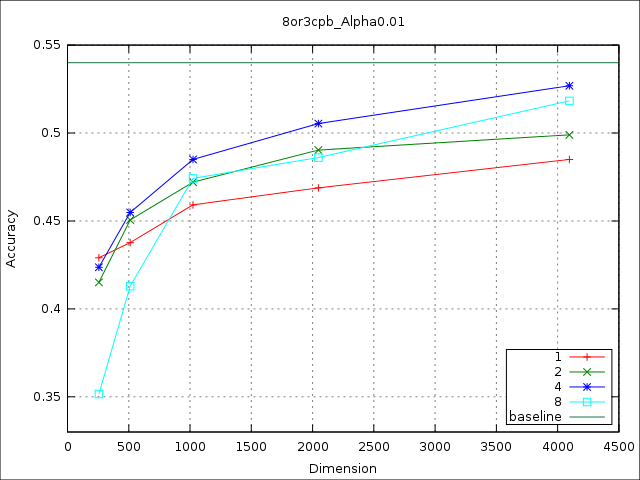
\includegraphics[scale=0.6]{img/resultados/reales/media_8or3cpb_Alpha0,01.png}
				\caption[Reales con umbral media]{Resultado de haber usado la media para la binarización de las características. La mejor clasificación se logra con los siguientes parámetros: \textit{alpha:0.01}, \textit{bits por grupo: 4}, \textit{dim del vector: 4096}, \textit{orientaciones: 8}, \textit{celdas por bloque: 9}.}
				\label{fig: Reales-media-8or9cpbAlph0.01}
			\end{figure}
			
			\begin{figure}[htbp]
				\centering
				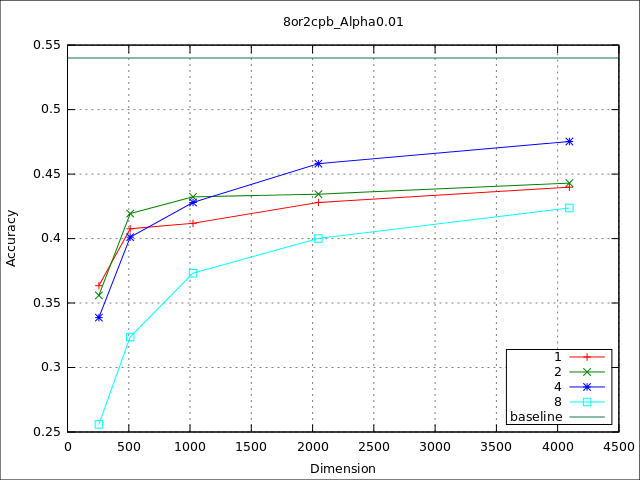
\includegraphics[scale=0.6]{img/resultados/reales/median_8or2cpb_Alpha0,01.png}
				\caption[Reales con umbral mediana]{Resultado de haber usado la mediana para la binarización de las características. La mejor clasificación se logra con los siguientes parámetros: \textit{alpha:0.01}, \textit{bits por grupo: 4}, \textit{dim del vector: 4096}, \textit{orientaciones: 8}, \textit{celdas por bloque: 4}.}
				\label{fig: Reales-mediana-8or4cpbAlph0.01}
			\end{figure}
			
			\begin{figure}[htbp]
				\centering
				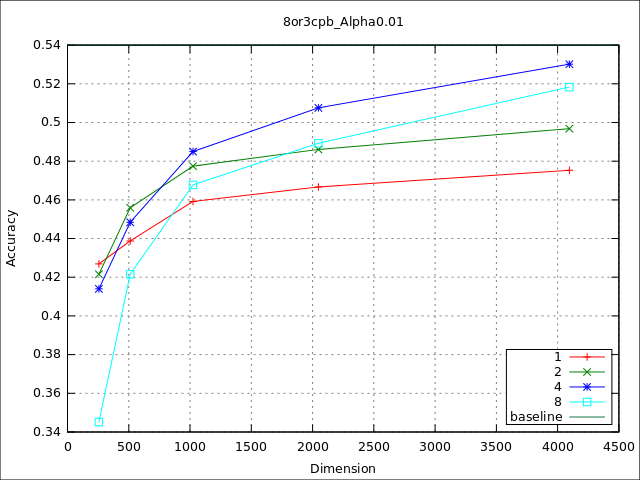
\includegraphics[scale=0.6]{img/resultados/reales/expon_8or3cpb_Alpha0,01.png}
				\caption[Reales con umbral exponencial]{Resultado de haber usado la distribución exponencial para la binarización de las características. La mejor clasificación se logra con los siguientes parámetros: \textit{alpha:0.01}, \textit{bits por grupo: 4}, \textit{dim del vector: 4096}, \textit{orientaciones: 8}, \textit{celdas por bloque: 9}.}
				\label{fig: Reales-expon-8or9cpbAlph0.01}
			\end{figure}
			
			\begin{figure}[htbp]
				\centering
				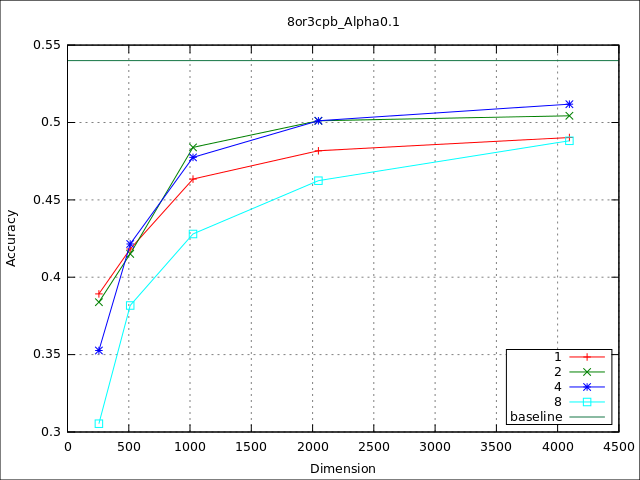
\includegraphics[scale=0.6]{img/resultados/reales/bootstrap_8or3cpb_Alpha0,1.png}
				\caption[Reales con umbral boostrap]{Resultado de haber usado bootstrap para la binarización de las características. La mejor clasificación se logra con los siguientes parámetros: \textit{alpha:0.1}, \textit{bits por grupo: 4}, \textit{dim del vector: 4096}, \textit{orientaciones: 8}, \textit{celdas por bloque: 9}.}
				\label{fig: Reales-bootstrap-8or9cpbAlph0.1}
			\end{figure}
			
			\begin{figure}[htbp]
				\centering
				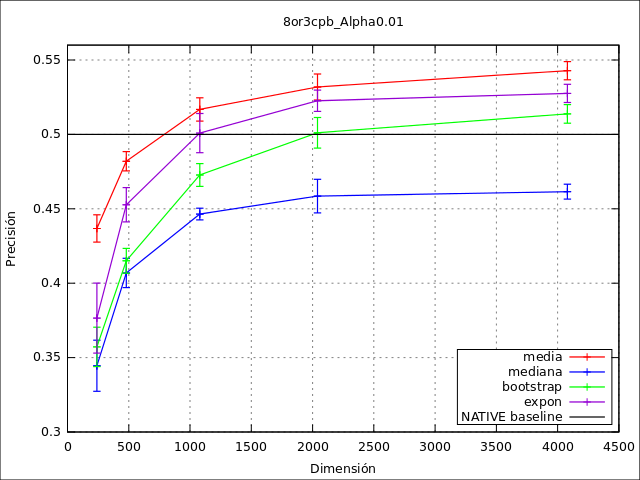
\includegraphics[scale=0.6]{img/resultados/reales/comparativa_metodos.png}
				\caption[Reales - Comparación entre métodos]{Este gráfico muestra las mejores curvas de los gráficos \ref{fig: Reales-media-8or9cpbAlph0.01}~\ref{fig: Reales-mediana-8or4cpbAlph0.01}~\ref{fig: Reales-expon-8or9cpbAlph0.01} y \ref{fig: Reales-bootstrap-8or9cpbAlph0.1}.}
				\label{fig: Reales-Comparativa metodos}
			\end{figure}

\newpage

		Se puede analizar en los cuatro experimentos realizados sobre imágenes reales, el mejor resultado se obtiene cuando se utilizan $4$ bits por grupo y la longitud de los vectores es de $4096$. También se puede observar que de los valores evaluados para alpha, el valor $0,01$ es el que se destaco por presentar los mejores resultados. Asi también, en la mayoría de los casos y más aún en el gráfico donde se utiliza el método exponencial, la mejor configuración para la cantidad de orientaciónes y celdas por bloque es $8$ y $9$ respectivamente. De los cuatro métodos propuestos para la binarización, el método exponencial y la media arrojan resultados muy similares como se puede observar en \ref{fig: Reales-Comparativa metodos}. La comparación final se puede observar en la tabla \ref{table: reales-comparativa}
	\begin{table}
		\centering
		\begin{tabular}{ | l | l | l | p{5cm} |}
    			\hline
    				\textbf{NATIVE + FERNS} & \textbf{Score} \\ \hline
    				Wang et al. & 0.54\% \\ \hline
    				Media & 0.53\% \\ \hline
    				Mediana & 0.47\%\\ \hline
    				Exponencial & 0.53\% \\ \hline
    				Bootstrap & 0.51\%\\ 
    			\hline
    		\end{tabular}
    		\caption[Resultados imagenes naturales vs Wang]{Tabla comparativa entre el resultado obtenido por Wang para imágenes naturales y los obtenidos en el presente trabajo, utilizando los cuatro umbrales propuestos.}
    		\label{table: reales-comparativa}
    	\end{table}
    	
    	
    	\newpage
    	\subsubsection{Imágenes Sintéticas}
    	
    En esta etapa se procederán mostrar los resultados obtenidos de los experimentos con las imágenes sintéticas. Vamos a comparar los valores conseguidos en estos con aquel logrado por Wang et al. que fue de $0.47$. Este último pasará a ser el nuevo \textit{baseline} en los gráficos a presentar. Además, los gráficos van a representar la relación entre la cantidad de imágenes sintéticas por clase (dado por \textit{IPC} en las siguientes figuras) y la precisión de clasificación dada por los $6$ valores a evaluar que son las dimensiones de los grupos. En estos experimentos, se decidió evaluar un rango más amplio de valores para las dimensiones de los grupos y observar los valores arrojados por el clasificador. Esto se realiza, con la finalidad de ver si hay un aumento en los valores a medida que se aumenta la dimensión de los grupos y observar que sucede por supuesto a medida que aumentamos la cantidad de imágenes po clase. Teniendo en cuenta los resultados anteriores con las imágenes reales, se decide por trabajar con $8$ orientaciones y $9$ celdas por bloque ya que son los parámetros que mejores resultados dieron. \RC{O también se puede aclarar que se experimentaron con los otros parámetros pero que 8 orientaciones y 9 celdas por bloque seguían arrojando los mejores resultados por lo cual se decidió trabajar con estos valores.}
    
    Las figuras que se presentan a continuación están organizadas de la siguiente manera. Se van a presentar de manera continua el mejor y el peor resultado para cada experimento utilizando uno de los métodos de binarización. Al final se realiza un pequeño resumen de los resultados, se presentará una tabla comparativa entre los valores arrojados en este trabajo y los conseguidos por Wang et al. Además, de la misma manera que se hizo para las imágenes reales, se va a incluir un gráfico con las mejores curvas de entre todos los gráficos presentados para que sea más fácil visualizar los mejores resultados.
\RC{Directamente podría omitir los métodos como la mediana o bootstrap que sé que no dan buenos resultados}

			\begin{figure}[htbp]
				\centering
				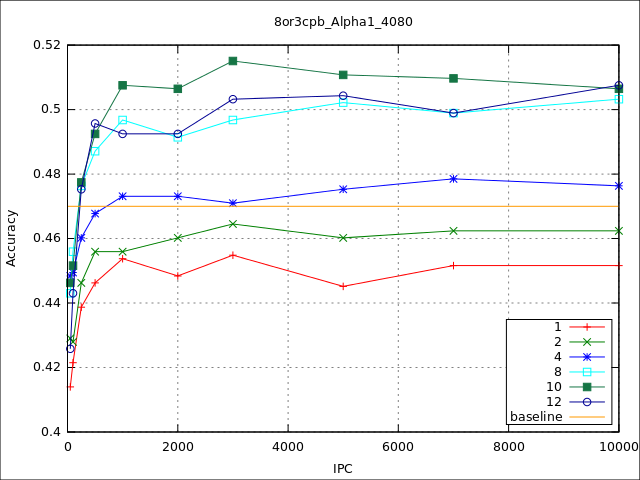
\includegraphics[scale=0.6]{img/resultados/sinteticas/best_media_8or3cpb_Alpha1_4080.png}
				\caption[Sintéticas media mejor resultado]{El gráfico muestra la configuración que devolvió los mejores resultados al utilizar la media en la binarización. Parámetros del mejor resultado: \textit{alpha:1}, \textit{IPC:3000}, \textit{dim grupo: 10}, \textit{dim vector: 4080}}
				\label{fig: Sinteticas-media-mejor}
			\end{figure}
			
			\begin{figure}[htbp]
				\centering
				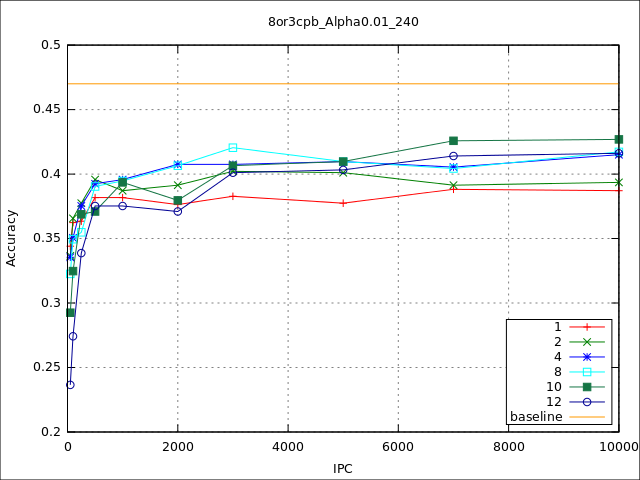
\includegraphics[scale=0.6]{img/resultados/sinteticas/worst_media_8or3cpb_Alpha0,01_240.png}
				\caption[Sintéticas media bajo resultado]{El gráfico muestra la configuración que devolvió los peores resultados al utilizar la media en la binarización. Parámetros del peor resultado: \textit{alpha:0.01}, \textit{IPC:50}, \textit{dim grupo: 12}, \textit{dim vector: 240}}
				\label{fig: Sinteticas-media-bajo}
			\end{figure}
			
			\begin{figure}[htbp]
				\centering
				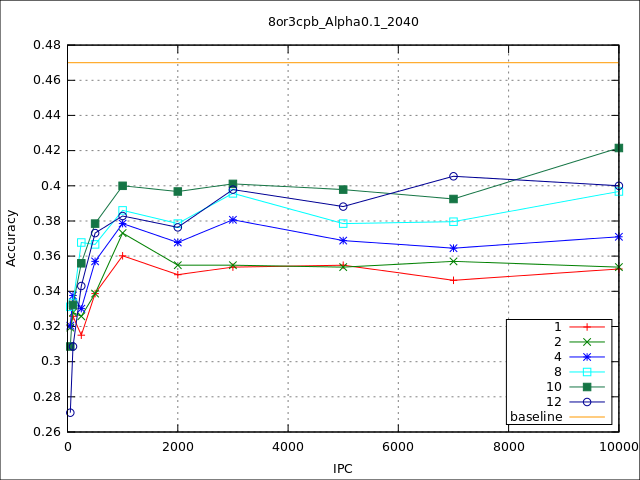
\includegraphics[scale=0.6]{img/resultados/sinteticas/best_median_8or3cpb_Alpha0,1_2040.png}
				\caption[Sintéticas mediana mejor resultado]{El gráfico muestra la configuración que devolvió los mejores resultados al utilizar la mediana en la binarización. Parámetros del mejor resultado: \textit{alpha:0.1}, \textit{IPC:10000}, \textit{dim grupo: 10}, \textit{dim vector: 2040}}
				\label{fig: Sinteticas-median-mejor}
			\end{figure}
	
			\begin{figure}[htbp]
				\centering
				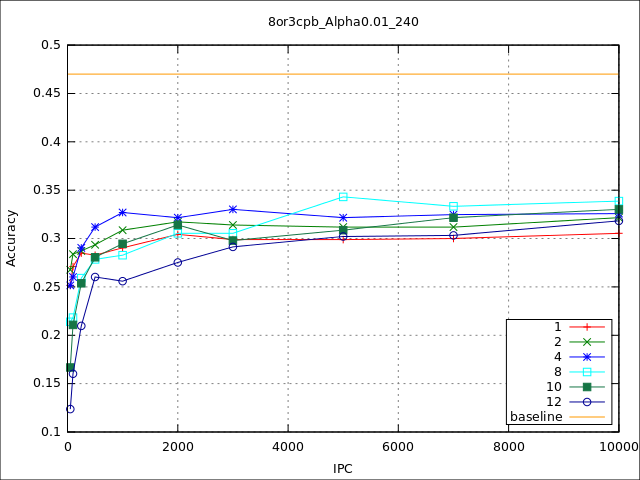
\includegraphics[scale=0.6]{img/resultados/sinteticas/worst_median_8or3cpb_Alpha0,01_240.png}
				\caption[Sintéticas mediana peor resultado]{El gráfico muestra la configuración que devolvió los peores resultados al utilizar la mediana en la binarización. Parámetros del peor resultado: \textit{alpha:0.01}, \textit{IPC:50}, \textit{dim grupo: 12}, \textit{dim vector: 240}}
				\label{fig: Sinteticas-median-bajo}
			\end{figure}
				
			\begin{figure}[htbp]
				\centering
				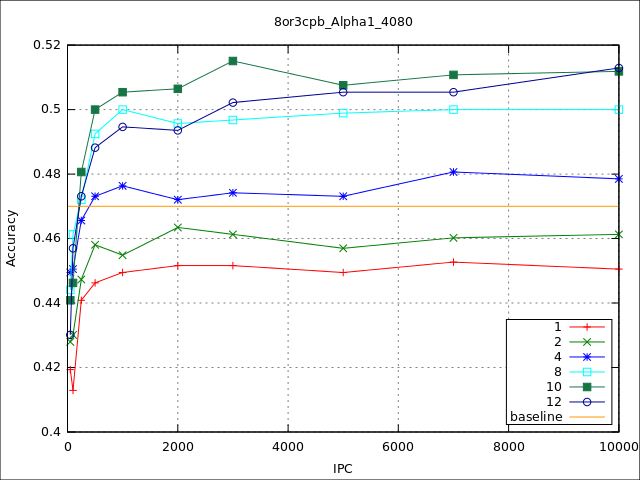
\includegraphics[scale=0.6]{img/resultados/sinteticas/best_expon_8or3cpb_Alpha1_4080.png}
				\caption[Sintéticas exponencial mejor resultado]{El gráfico muestra la configuración que devolvió los mejores resultados al utilizar la distribución exponencial en la binarización. Parámetros del mejor resultado: \textit{alpha:1}, \textit{IPC:3000}, \textit{dim grupo: 10}, \textit{dim vector: 4080}}
				\label{fig: Sinteticas-expon-mejor}
			\end{figure}
	
			\begin{figure}[htbp]
				\centering
				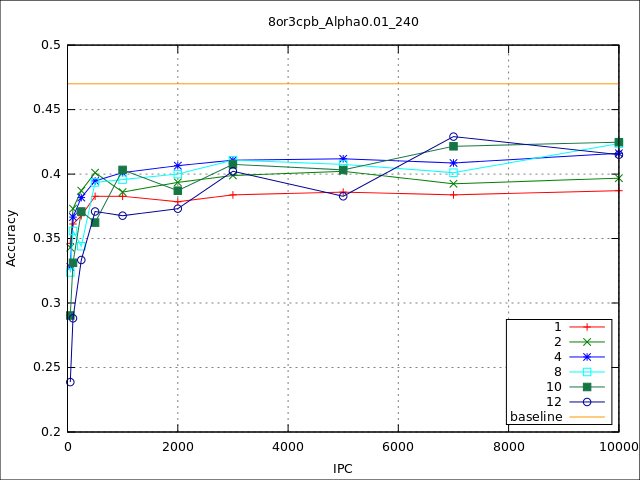
\includegraphics[scale=0.6]{img/resultados/sinteticas/worst_expon_8or3cpb_Alpha0,01_240.png}
				\caption[Sintéticas exponencial peor resultado]{El gráfico muestra la configuración que devolvió los peores resultados al utilizar la distribución exponencial en la binarización. Parámetros del peor resultado: \textit{alpha:0.01}, \textit{IPC:50}, \textit{dim grupo: 12}, \textit{dim vector: 240}}
				\label{fig: Sinteticas-expon-bajo}
			\end{figure}
			
			\begin{figure}[htbp]
				\centering
				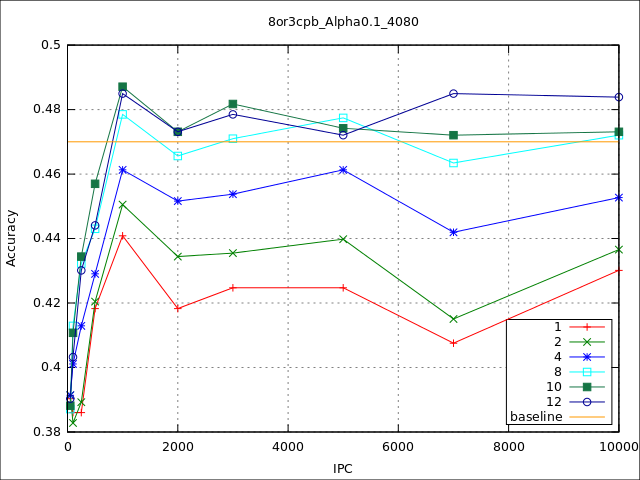
\includegraphics[scale=0.6]{img/resultados/sinteticas/best_bootstrap_8or3cpb_Alpha0,1_4080.png}
				\caption[Sintéticas bootstrap mejor resultado]{El gráfico muestra la configuración que devolvió los mejores resultados al utilizar bootstrap en la binarización. Parámetros del mejor resultado: \textit{alpha:0.1}, \textit{IPC:1000}, \textit{dim grupo: 10}, \textit{dim vector: 4080}}
				\label{fig: Sinteticas-bootstrap-mejor}
			\end{figure}
	
			\begin{figure}[htbp]
				\centering
				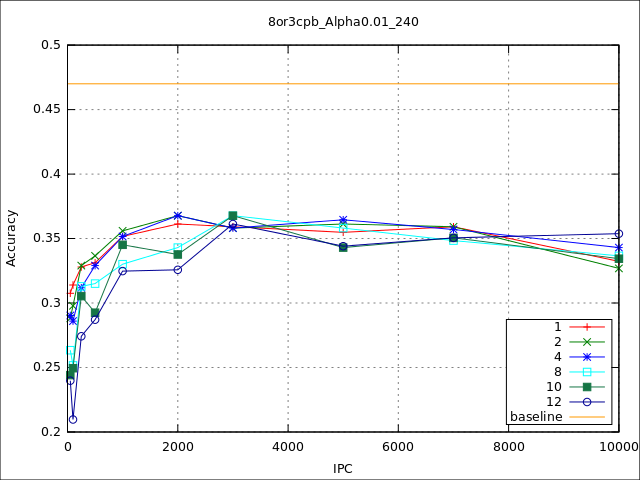
\includegraphics[scale=0.6]{img/resultados/sinteticas/worst_bootstrap_8or3cpb_Alpha0,01_240.png}
				\caption[Sintéticas bootstrap peor resultado]{El gráfico muestra la configuración que devolvió los peores resultados al utilizar bootstrap en la binarización. Parámetros del peor resultado: \textit{alpha:0.01}, \textit{IPC:50}, \textit{dim grupo: 12}, \textit{dim vector: 240}}
				\label{fig: Sinteticas-bootstrap-bajo}
			\end{figure}
			
			\begin{figure}[htbp]
				\centering
				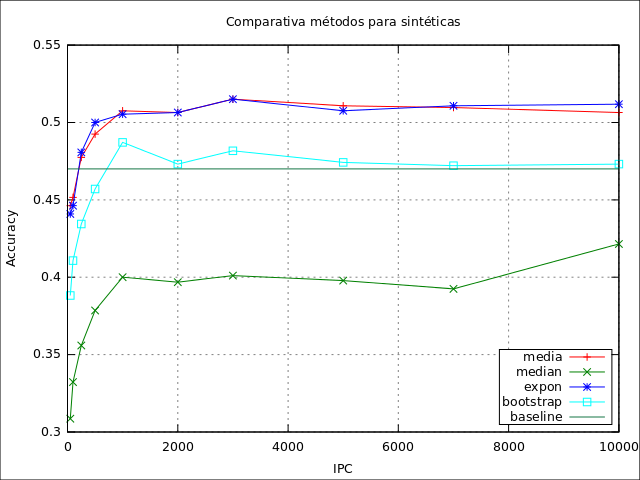
\includegraphics[scale=0.6]{img/resultados/sinteticas/comparativa_metodos.png}
				\caption[Sintéticas comparativa métodos]{El gráfico muestra las mejores curvas de los gráficos de cada método. \ref{fig: Sinteticas-media-mejor}~\ref{fig: Sinteticas-median-mejor}~\ref{fig: Sinteticas-expon-mejor} y \ref{fig: Sinteticas-bootstrap-mejor}}
				\label{fig: Sinteticas-comparativa metodos}
			\end{figure}

\newpage

	Hacer texto con las siguientes ideas
	\begin{itemize}
		\item En los experimentos con imágenes sintéticas en general a más cantidad de imágenes por clase mayor es la performance de clasificación. Sin embargo llega un punto en que se deja de aumentar la perfomances y en varios casos disminuye despues de cierto punto.
		\item Es claro que para este tipo de experimentos es mejor tener grupos de dimensiones mayores a los propuestos para las imágenes reales. Analizar que los casos donde los grupos tienen 12 bits la performance decae a comparación de los casos donde los mismo tienen 10 bits.
		\item Defenitivamente la mediana y bootstrap no son buenos métodos para binarizar.
	\end{itemize}

	\begin{table}
		\centering
		\begin{tabular}{ | l | l | l | p{5cm} |}
    			\hline
    				\textbf{SINT(1000) + FERNS} & \textbf{Score} \\ \hline
    				Wang et al. & 0.47\% \\ \hline
    				Media & 0.51\% \\ \hline
    				Mediana & 0.4\%\\ \hline
    				Exponencial & 0.5\% \\ \hline
    				Bootstrap & 0.49\%\\ 
    			\hline
    		\end{tabular}
    		\caption[Resultados imágenes sintéticas vs Wang]{Tabla comparativa entre el resultado obtenido por Wang para imágenes sintéticas y los obtenidos en el presente trabajo, utilizando los mejores resultados entre los cuatro umbrales propuestos. Se consideran para poder realizar la comparación los resultados cuando se evalua al clasificador con 1000 imágenes sintéticas.}
    	\end{table}
			
\newpage
    	\subsubsection{Imágenes Reales y Sintéticas}
    	
	Por último se van a mostrar los resultados correspondientes de haber entrenado al clasificador con conjuntos de entrenamiento mixtos. Se procederá a mostrar los gráficos con las mejores y peores configuraciones y sus resultados. También se mostrarán las matrices de correlación para todos estos casos. Teniendo en cuenta los resultados anteriores, se van a mostrar los resultados de haber utilizado solamente la distribución exponencial como umbral ya que fue la que obtuvo los mejores resultados. En los gráficos  se van a mostrar también los baselines de Wang et al. para las imágenes reales y las sintéticas.
	
			\begin{figure}[htbp]
				\centering
				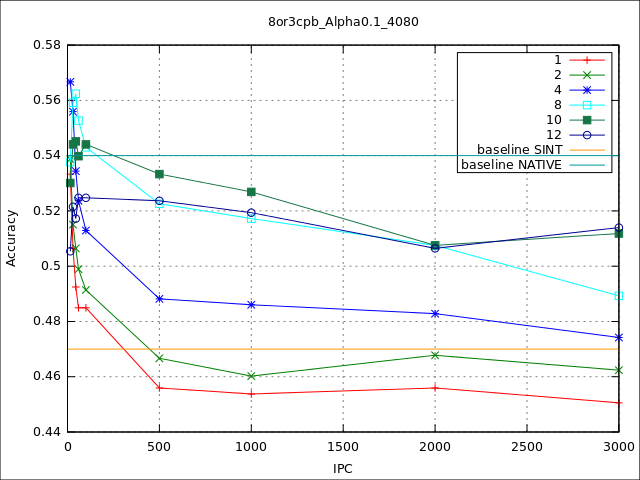
\includegraphics[scale=0.6]{img/resultados/mixtas/best_expon_8or3cpb_Alpha0,1_4080.png}
				\caption[Mixtas expon mejor resultado]{El gráfico muestra la configuración que devolvió los mejores resultados.}
				\label{fig: Mixtas-expon-mejor}
			\end{figure}

			\begin{figure}[!htbp]
				\centerline{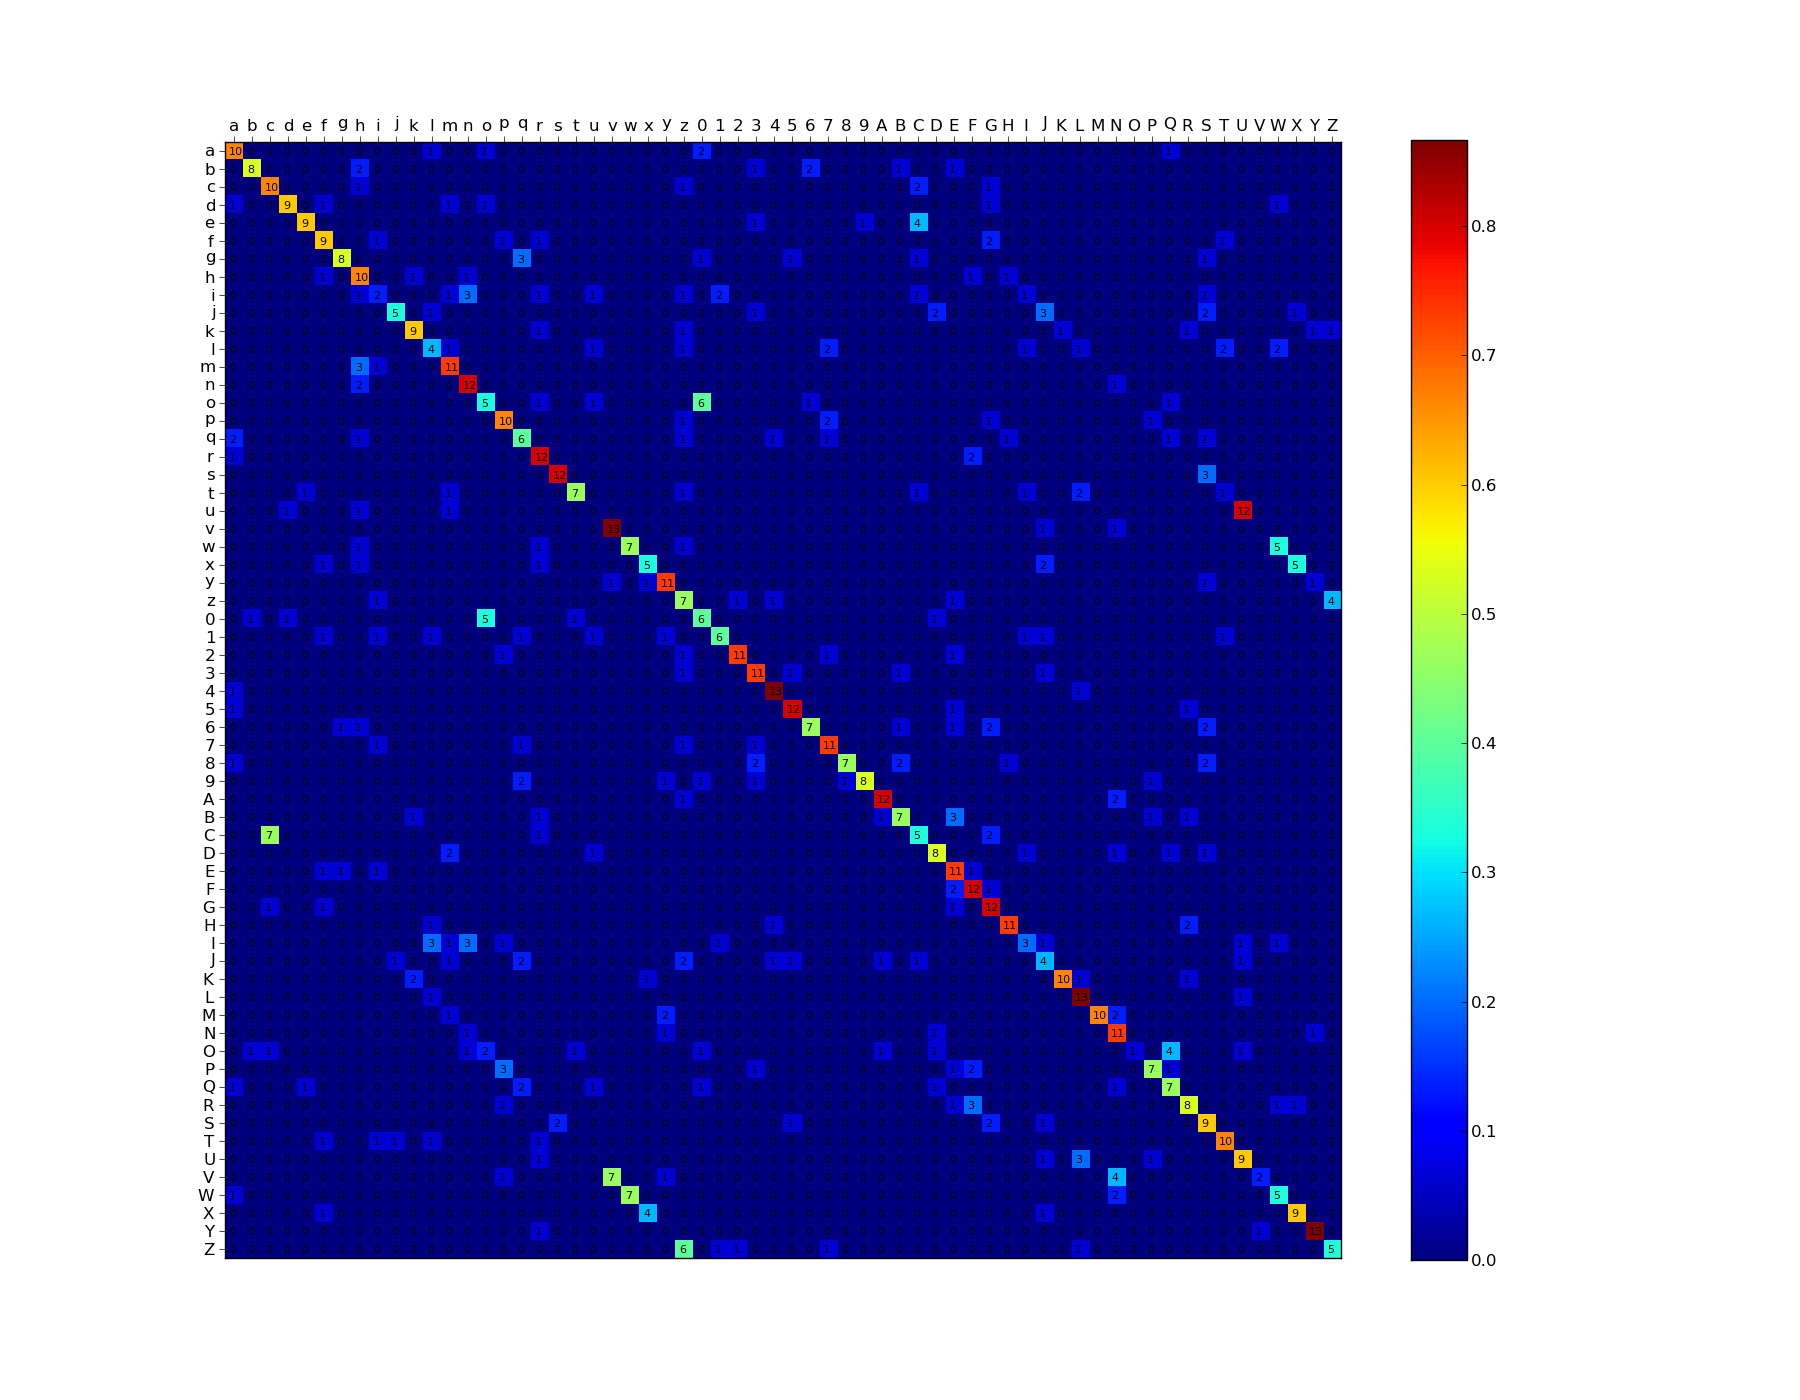
\includegraphics[scale=0.4]{img/resultados/mixtas/best_expon_matrix_Alpha0,1_4080-4.png}}
				\caption[Mixtas Matriz expon]{Matriz de correlación del gráfico \ref{fig: Mixtas-expon-mejor} para el mejor resultado. \RC{Demasiado grande las matrices como para mostrarlas y que se vean bien}}
				\label{fig: Mixtas-Matrix-expon-mejor}
			\end{figure}
	
			\begin{figure}[htbp]
				\centerline{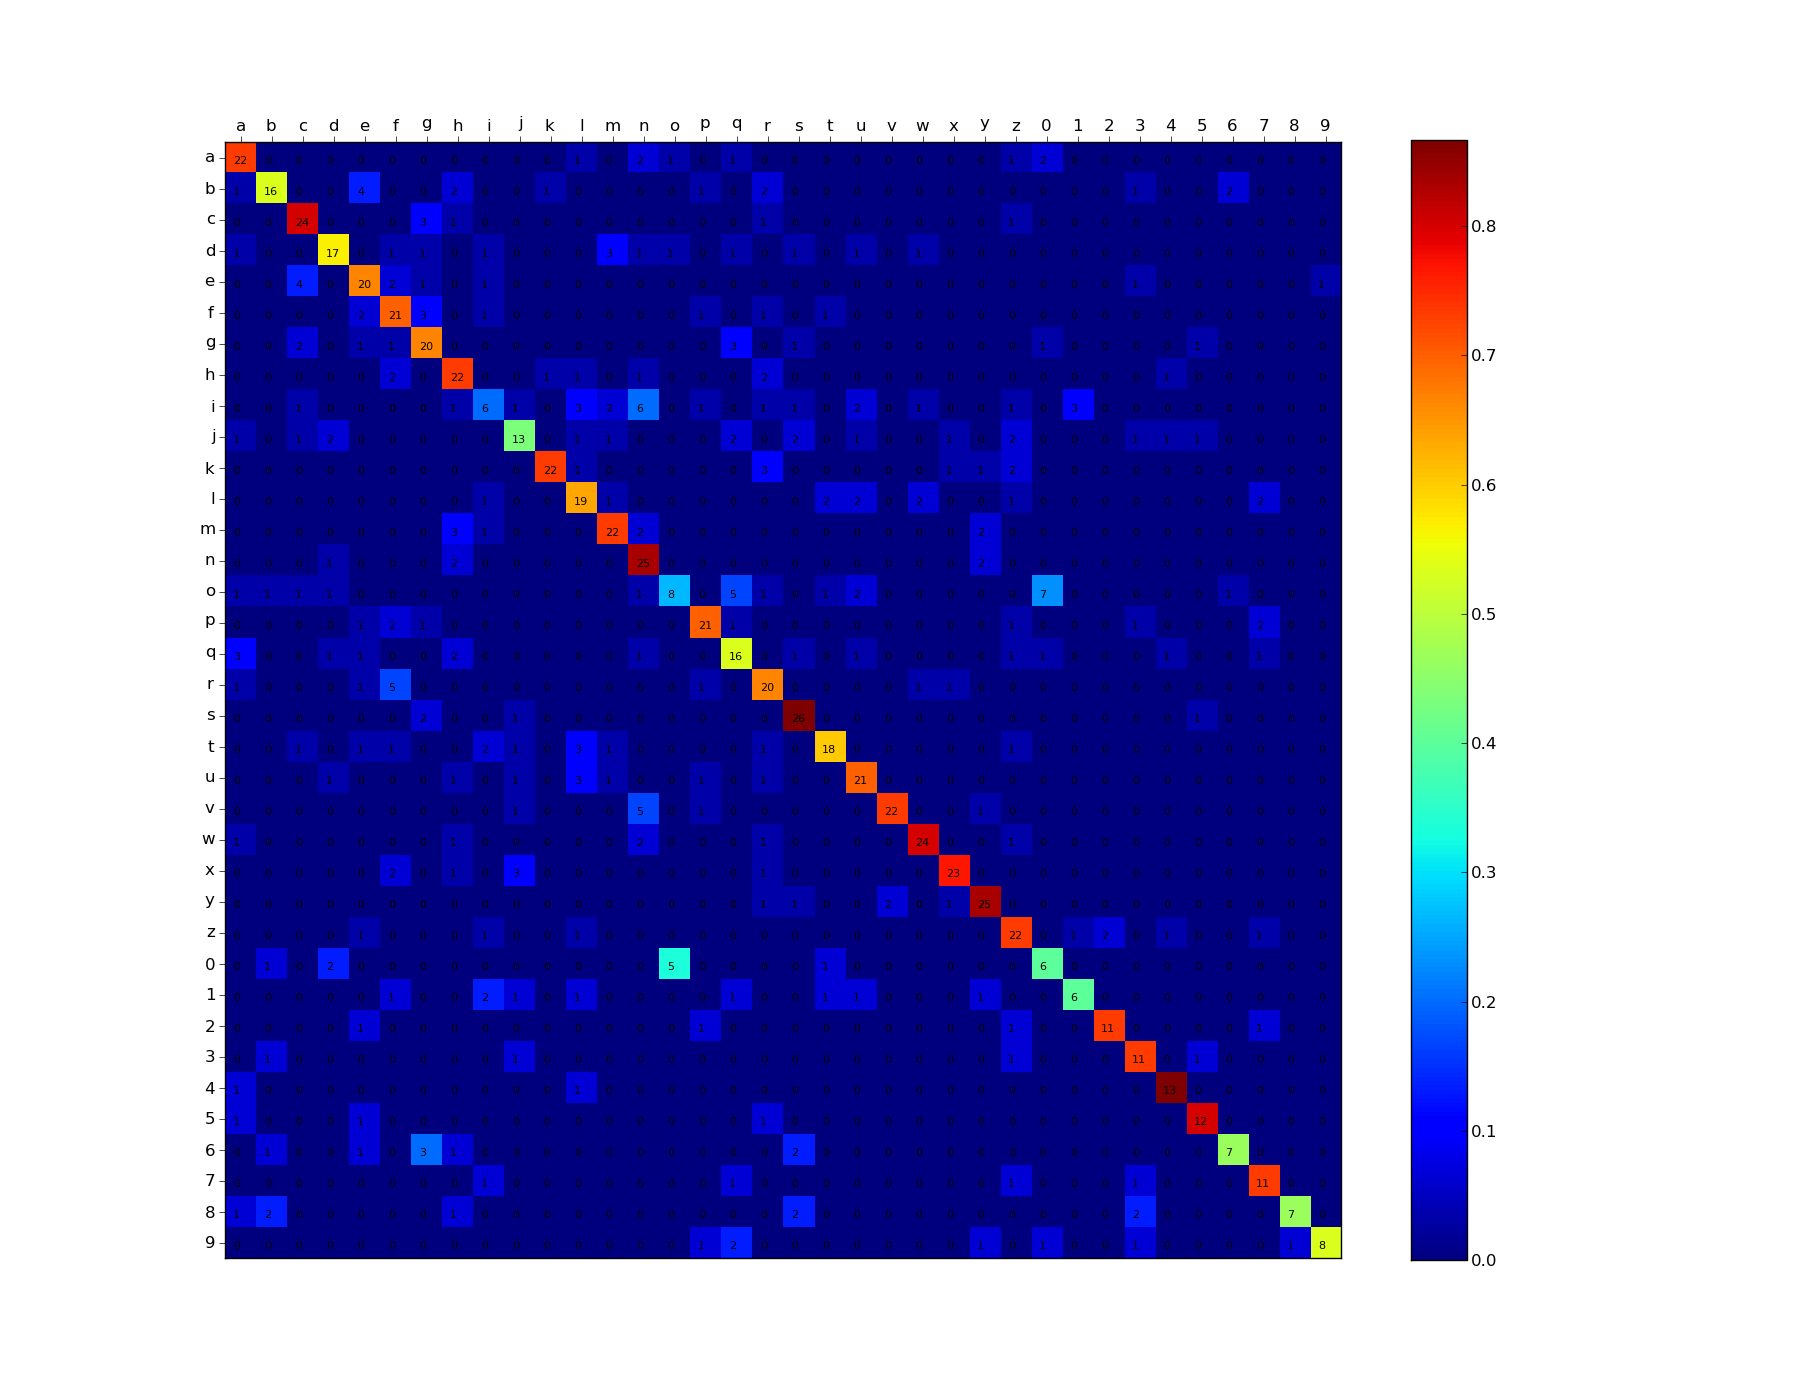
\includegraphics[scale=0.4]{img/resultados/mixtas/best_expon_matrix_Alpha0,1_4080-4_ins.png}}
				\caption[Matriz de correlación ``case insensitive'' para mixtas expon]{Matriz de correlación del gráfico \ref{fig: Mixtas-expon-mejor} para el mejor resultado no teniendo en cuenta los caracteres en mayúscula.}
				\label{fig: MatrizIns-Mixtas-expon}
			\end{figure}
	
    	\subsubsection{Comparativa}

    	\FL{Incluir gráfica que superpone las mejores curvas de cada sección anterior y Wang.}
    	